%+================+
%| DOCUMENT SETUP |
%+================+

% Set document class
\documentclass[xcolor=dvipsnames]{beamer}

% Include packages
% Encryption and spelling
\usepackage[utf8]{inputenc}
\usepackage[T1]{fontenc}
\usepackage[ngerman]{babel}

% Font type
\usepackage{DejaVuSansMono}	% Replaces original typewriter font

% Drawings and color
\usepackage{graphicx}
\usepackage{tikz}
\usepackage{xcolor}

% Formatting packages
\usepackage{listings}	% For code listings
\usepackage{fancyhdr}	% For footer/header settings
\usepackage{chngcntr}	% Stops resetting footnote counter
\usepackage{float}			% For fixed image positioning
\usepackage{svg}	% For SVG images

\lstdefinelanguage{javascript}{
  keywords={abstract, public, break, case, catch, continue, debugger, default, delete, do, else, finally, for, function, if, in, instanceof, new, null, return, switch, throw, try, typeof, var, void, while, with},
  keywords={[2]{class, export, boolean, String, Date, Infinity, Number, throw, implements, import, this, undefined, false, true, byte, int, document}},
  sensitive=false,
  comment=[l]{//},
  morecomment=[s]{/*}{*/},
  morestring=[b]',
  morestring=[b]"
}
\lstdefinelanguage{svg}{
	alsoletter=-,
	keywords={svg, circle, line, polygon, rectangle},
	keywords={[2]{width, height, viewBox, cx, cy, r, x1, x2, y1, y2, xmlns, stroke-width, stroke-linecap, stroke-linejoin, stroke, fill}},
	sensitive=false,
	comment=[l]{//},
	morecomment=[s]{/*}{*/}
	morestring=[b]',
	morestring=[b]"
}
\lstdefinelanguage{json}{
    sensitive=false,
    morestring=[b]',
    morestring=[b]",
    literate=
    {[}{{\color{red}\[}}1
}

\lstnewenvironment{code}[1][]{
	\lstset{
		#1,
		captionpos=b,
		backgroundcolor=\color{white},
		basicstyle=\footnotesize\ttfamily,
		commentstyle=\color{cyan}\itshape,
		keywordstyle=[1]\color{red}\bfseries,
		keywordstyle=[2]\color{violet}\bfseries,
		numberstyle=\color{black},
		stringstyle=\color{gray},
		breakatwhitespace=true,
		breaklines=true,
		keepspaces=true,
		numbers=left,
		numbersep=7pt,
		showspaces=false,
		showstringspaces=true,
		showtabs=false,
		tabsize=2,
		frame=l,
		extendedchars=true,
		literate=
		{Ö}{{\"O}}1
		{Ä}{{\"A}}1
		{Ü}{{\"U}}1
		{ß}{{\ss}}2
		{ü}{{\"u}}1
		{ä}{{\"a}}1
		{ö}{{\"o}}1
		{~}{{\textasciitilde}}1
	}
}{}		% Code style setup

%+----------------+
%| Document style |
%+----------------+

% Set default font to sans-serif
\renewcommand*{\familydefault}{\sfdefault}
% Make monospaced font a little smaller to fit text size
\let\tt\ttfamily
\renewcommand*{\ttfamily}{\small\tt}

\usetheme{Dresden}
\usecolortheme{beaver}

% Set author and title
\title[PSS isys vision]{Praxissemester bei isys vision GmbH \& Co. KG}
\subtitle{Bericht und Erfahrungen}
\author{Lorenz Bung}
\date{01. März 2018 bis 31. Juli 2018}

%+================+
%| DOCUMENT START |
%+================+
\begin{document}

%+------------+
%| Title page |
%+------------+
\frame{\titlepage}
\begin{frame}{Gliederung}
\tableofcontents
\end{frame}


\section{Motivation}

\begin{frame}{Meine Motivation}
\begin{itemize}
\item Entscheidung für Vertiefung Medieninformatik
\item Bildverarbeitung, -generierung oder Web-Development
\item Standort in Baden-Württemberg
\end{itemize}
\end{frame}


\section{Das Unternehmen}

\begin{frame}{Über isys vision}
\begin{figure}[t]

\includegraphics[height=0.1\textheight]{media/isys.png}
\end{figure}
\begin{itemize}
\item Mittelständisches Unternehmen mit ca. 20 Mitarbeitern
\item Fokus auf industrieller Bildverarbeitung
\item Standort in Freiburg im Breisgau
\item Zulieferer für Bosch und Omron
\end{itemize}
\end{frame}

\begin{frame}{Produkte}
\begin{columns}
\begin{column}{0.6\textwidth}
\begin{itemize}
\item Bildverarbeitungssysteme für die Industrie
\item z.B. Ausrichtungen für Lotpasten oder Fräsungen
\item Robotikprojekt Mikado
\begin{itemize}
\item ``Bin-Picking'': Griff in die Kiste
\item graphische Programmierung für Endkunden
\end{itemize}
\item Visionsysteme für Druck- und Lasermaschinen
\end{itemize}
\end{column}
\begin{column}{0.4\textwidth}
\begin{figure}[t]
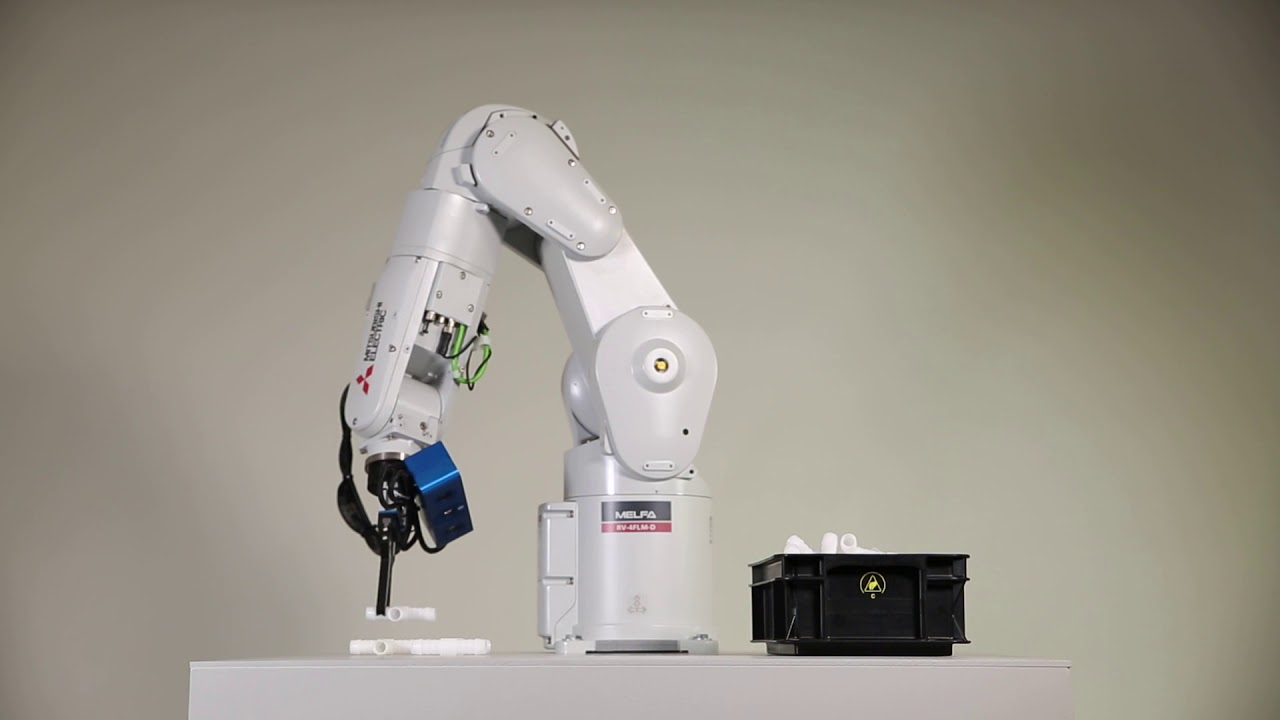
\includegraphics[width=\textwidth]{media/mikado-roboter.jpg}
\caption{Mikado Robotik-System}
\end{figure}
\end{column}
\end{columns}
\end{frame}


\section{Das Praktikum}

\begin{frame}{Aufarbeitung einer Weboberfläche}
\begin{itemize}
\item Grafisches Redesign des Interfaces
\item Anpassen der Funktionalität
\end{itemize}
\begin{figure}[t]
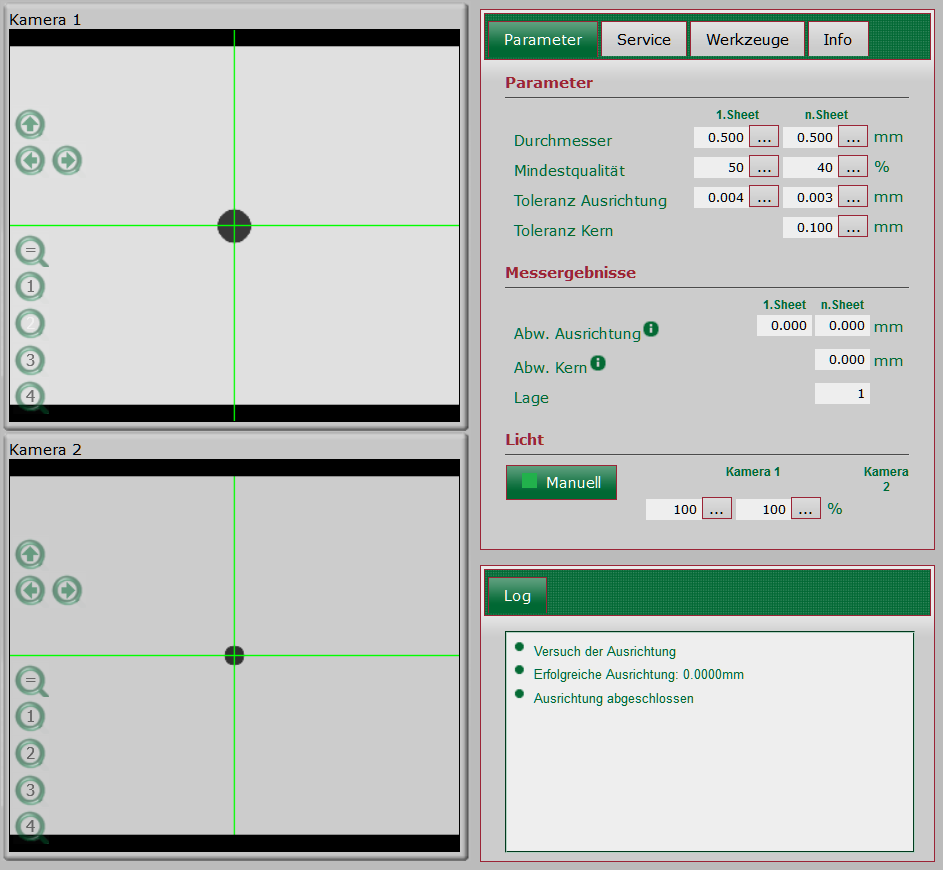
\includegraphics[width=0.4\textwidth]{media/webinterface-alt.png}
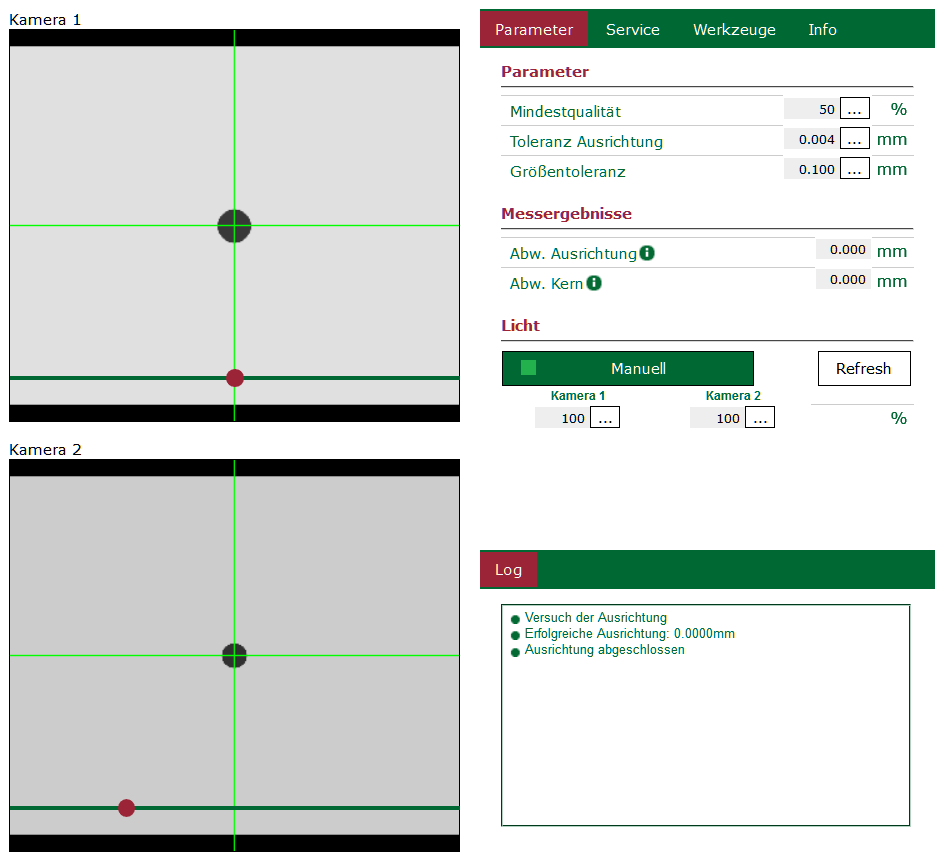
\includegraphics[width=0.4\textwidth]{media/webinterface.png}
\end{figure}
\end{frame}

\begin{frame}{Einrichtung eines Intranet-Servers}
\begin{itemize}
\item Jira und Confluence für das Produktionsmanagement
\item vollständig neuer Intranetserver
\begin{itemize}
\item Datenbank mit PostgreSQL
\item RAID5 zur Datensicherung
\end{itemize}
\item Linux-Systemadministration
\end{itemize}
\end{frame}

\begin{frame}{Mikado: WebRemote}
\begin{columns}
\begin{column}{0.7\textwidth}
\begin{itemize}
\item Webtool zur Kontrolle per Smartphone
\item Responsive Design für automatische Anpassung
\item Kommunikation durch ROS\footnotemark[1]
\item Erstellung von SVG-Grafiken
\end{itemize}
\end{column}
\begin{column}{0.3\textwidth}
\begin{figure}[t]
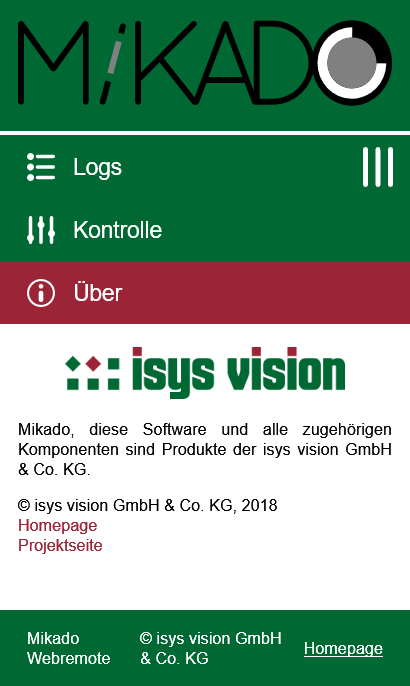
\includegraphics[width=\textwidth]{media/webremote-info.png}
\end{figure}
\end{column}
\end{columns}
\footnotetext[1]{Roboter Operating System}
\end{frame}

\begin{frame}{Mikado: WebPreview}
\begin{figure}[t]
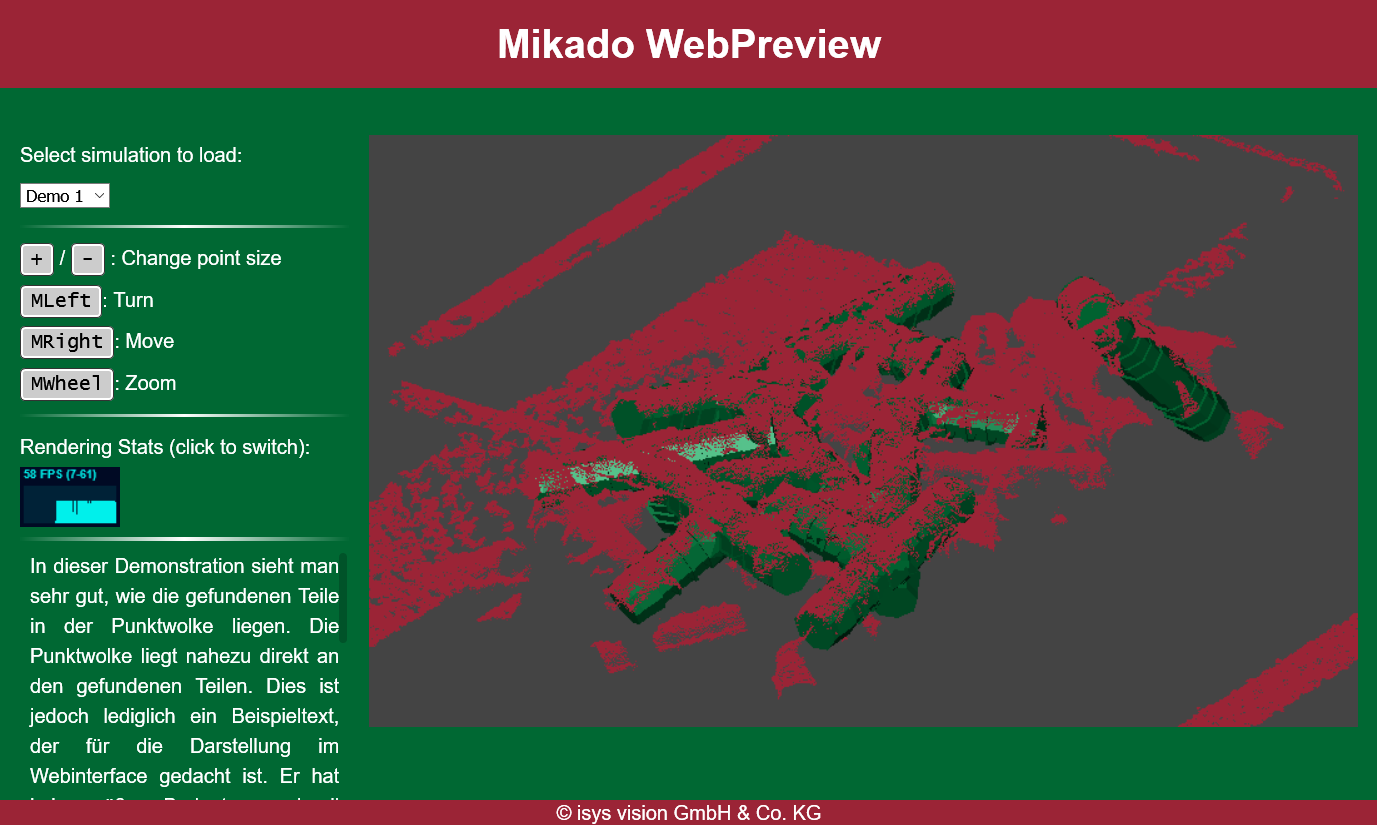
\includegraphics[width=0.5\textwidth]{media/webpreview.png}
\end{figure}
\begin{itemize}
\item Vorschau von gefundenen Teilen in Punktewolke
\item Einlesen von JSON-Dateien und Modelldaten
\item Animation mit \texttt{THREE.js}
\end{itemize}
\end{frame}

\begin{frame}{Verwendete Technologien}
\begin{itemize}
\item Javascript
\begin{itemize}
\item jQuery, jQuery UI
\item Node.js, THREE.js, Roslib.js
\end{itemize}
\item CSS, HTML
\item Linux-Tools, \texttt{mdadm}
\item PostgreSQL
\item JSON, SVG
\item Subversion
\end{itemize}
\end{frame}


\section{Das soziale Umfeld}

\begin{frame}
\end{frame}


\section{Fazit}

\begin{frame}{Bilanz und Empfehlung}
\end{frame}


%+==============+
%| DOCUMENT END |
%+==============+
\end{document}